\documentclass{article}[letterpaper]
\usepackage{float}
\usepackage{geometry}
\geometry{letterpaper, margin=2.54cm}
\usepackage{graphicx}
\usepackage{anysize}
\usepackage{geometry}
\usepackage{lipsum}
\usepackage{amsmath,amssymb,amsthm}
\usepackage[utf8]{inputenc}
\usepackage{multirow}
\usepackage{csquotes}
\usepackage[spanish]{babel}
\usepackage{apacite}
\usepackage{multicol}
\usepackage{parskip}
\usepackage{setspace}
\doublespacing
\begin{document}
\begin{titlepage}
\centering


\vspace{0.5cm}
{\scshape\Huge Trabajo de Dinámica \par}
\vspace{3cm}
\textbf\large\scshape{\par}
     \vspace{4cm}
     
{\Large Vergara Pareja Gustavo\\Pacheco Berrio Jhosuea\\Petro Yanéz Edwin\par}
\vspace{6cm}
{\scshape\Large Programa de Ingeniería Mecánica \par}
\vspace{0.5cm}
{\scshape\Large Universidad de Córdoba\par}
\vspace{0.5cm}
{\Large \today \par}
\end{titlepage}

\newpage
\tableofcontents
\newpage

\section*{Introducción}
\addcontentsline{toc}{section}{Introducción}
Una troqueladora manual es una herramienta de trabajo utilizada en la industria para cortar, perforar o doblar materiales como papel, cartón, plástico o metal. Esta máquina funciona mediante la aplicación de una fuerza mecánica que activa un troquel, una herramienta de corte o moldeado que corta o da forma al material.
 \newline 
 El objetivo es determinar las características de velocidad y aceleración de la máquina. Para ello, se realizarán simulaciones y cálculos utilizando análisis dinámico y los modelos 3D de la troqueladora.
Se responderán preguntas 
como: ¿Cómo se diseñó la troqueladora?, ¿Con qué materiales se construyó? y ¿Cuál es su finalidad?.
\newline
Para lograr este objetivo, se utilizarán principios de la física y la mecánica para describir
 el movimiento de la troqueladora y se analizarán las fuerzas involucradas en su funcionamiento. 
 Además, se describirá el diseño mecánico de esta, incluyendo los materiales utilizados 
 y las especificaciones técnicas.
 \newpage

\section*{¿Qué se hizo?}
\addcontentsline{toc}{section}{¿Qué se hizo?}

El objetivo de este proyecto fue estudiar el movimiento de una troqueladora y realizar cálculos empíricos
 de su velocidad, aceleración y análisis de fuerzas. En la práctica, se construyó una troqueladora manual y se realizaron experimentos para medir. \begin{itemize}
    \item El tiempo que tarda en cortar una pieza.
    \item Demostrar conceptos de dinámica como la aceleración, la velocidad y la gravedad que afectan a la máquina.
 \end{itemize}

\section*{Materiales y métodos}
\addcontentsline{toc}{section}{Materiales y métodos}
Los materiales utilizados para el desarrollo de esttroqueladora fueron:

\begin{itemize}
  \item Madera
  \item Carton
  \item Tornillos
  \item Clavos
  \item Caucho
  \item Silicona
  \item Botella en lata
\end{itemize}
\newpage
\section*{Contenido y Resultados}
\addcontentsline{toc}{section}{Contenido y Resultados}
Para el desarrollo de este proyecto, hicimos una busqueda exhaustiva de modelos e ideas para construir la maquina:
\begin{figure}[H]
\centering
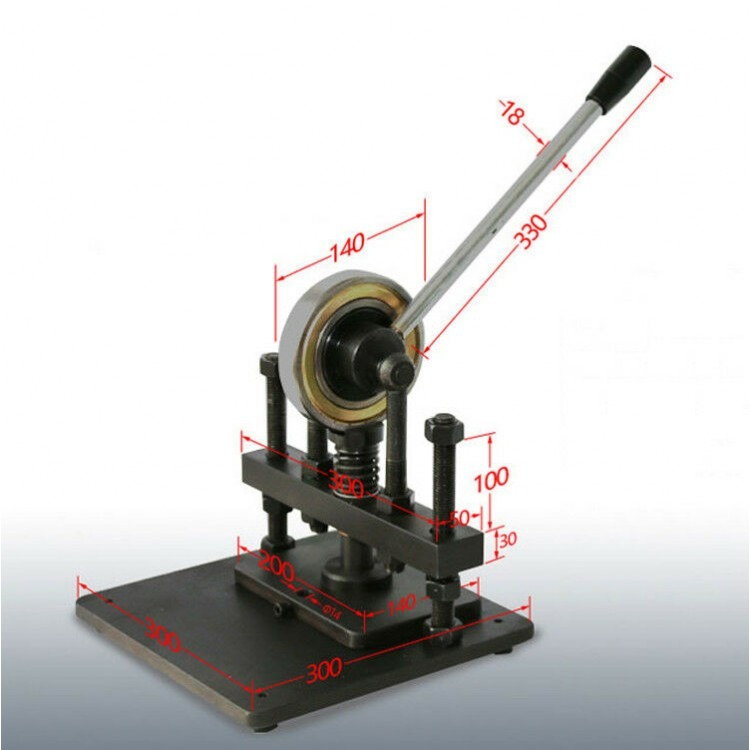
\includegraphics[width=0.5\textwidth]{modelo.jpg}
\caption{Modelo de Troqueladora comercial}
\label{fig:imagen}
\end{figure}
\begin{itemize}
\item Luego de esto, pasamos a hacer mediciones y cálculos empíricos:
\end{itemize}
\begin{figure}[H]
\centering
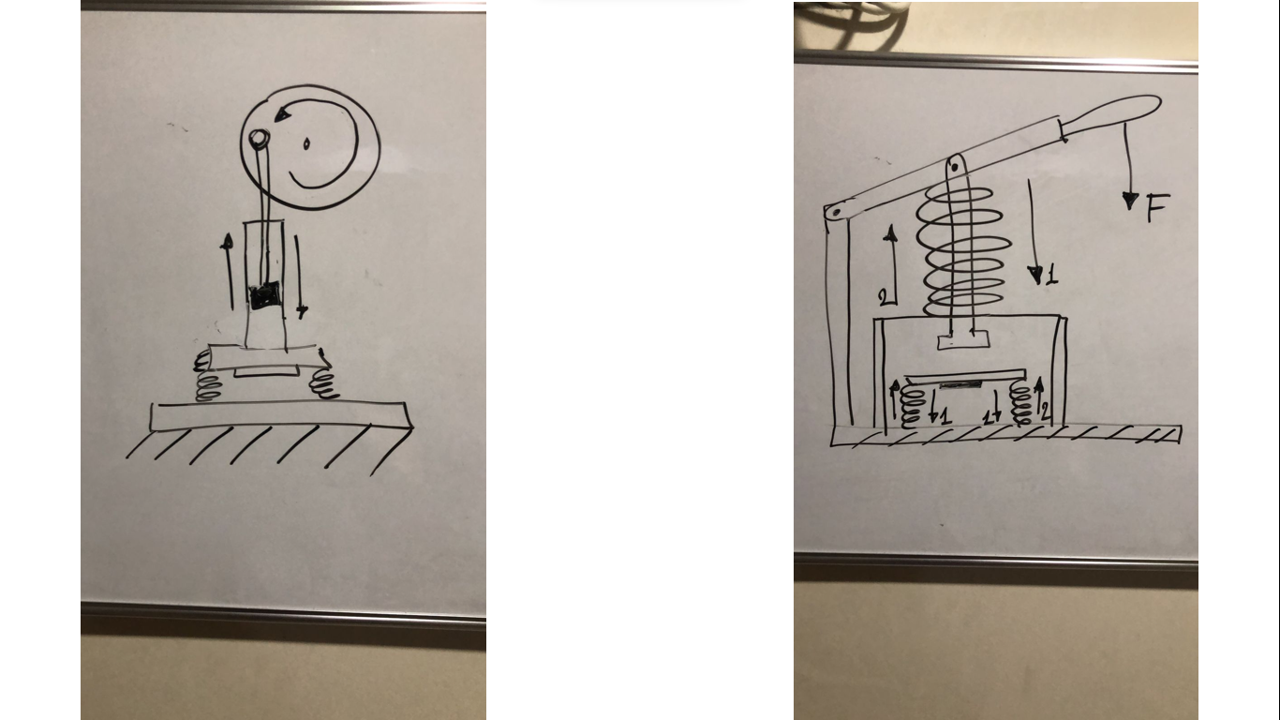
\includegraphics[width=0.8\textwidth]{calculitos.png}
\caption{Diseños a mano}
\label{fig:imagen1}
\end{figure}
\newpage
\begin{itemize}
\item Desarrollo de la troqueladora
\end{itemize}
\begin{figure}[H]
    \centering
    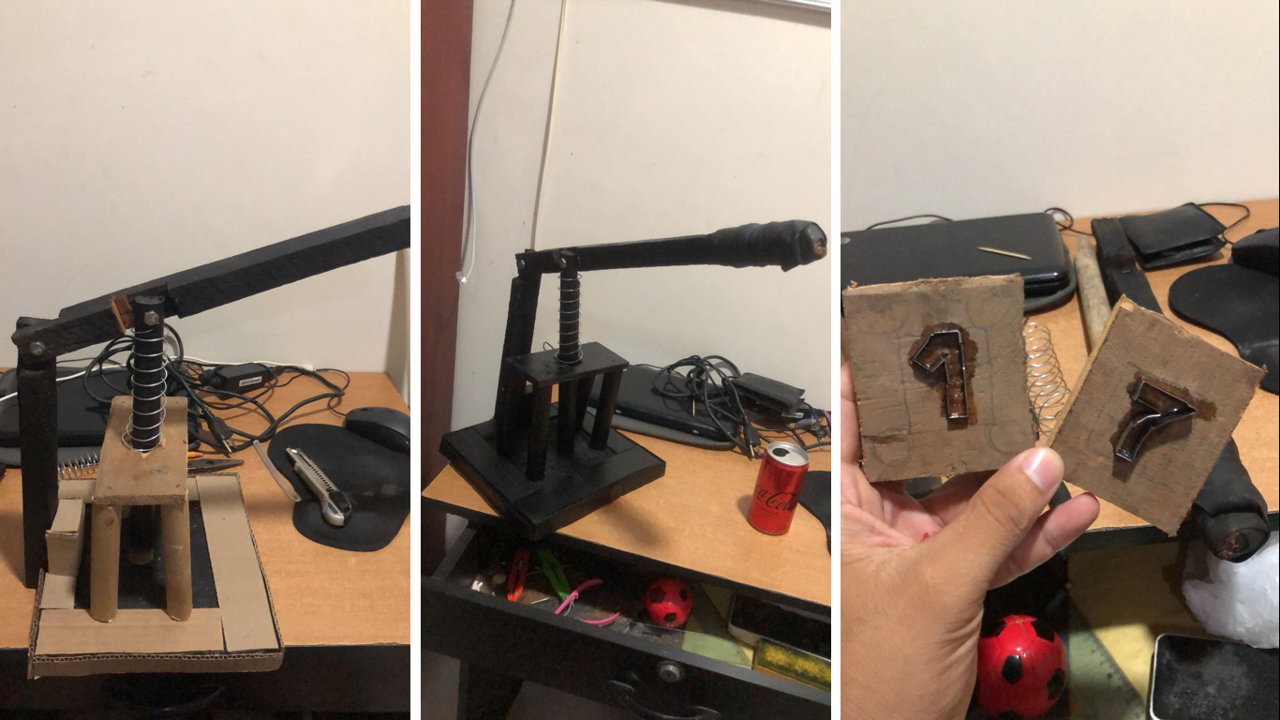
\includegraphics[width=0.8\textwidth]{finish.png}
    \caption{Fases de la Troqueladora}
    \label{fig:imagen2}
  \end{figure}  
    \begin{itemize}
    \item Para el análisis dinámico, nos apoyamos de herramientas de SolidWorks.
    \end{itemize}
    \begin{figure}[H]
    \centering
    
    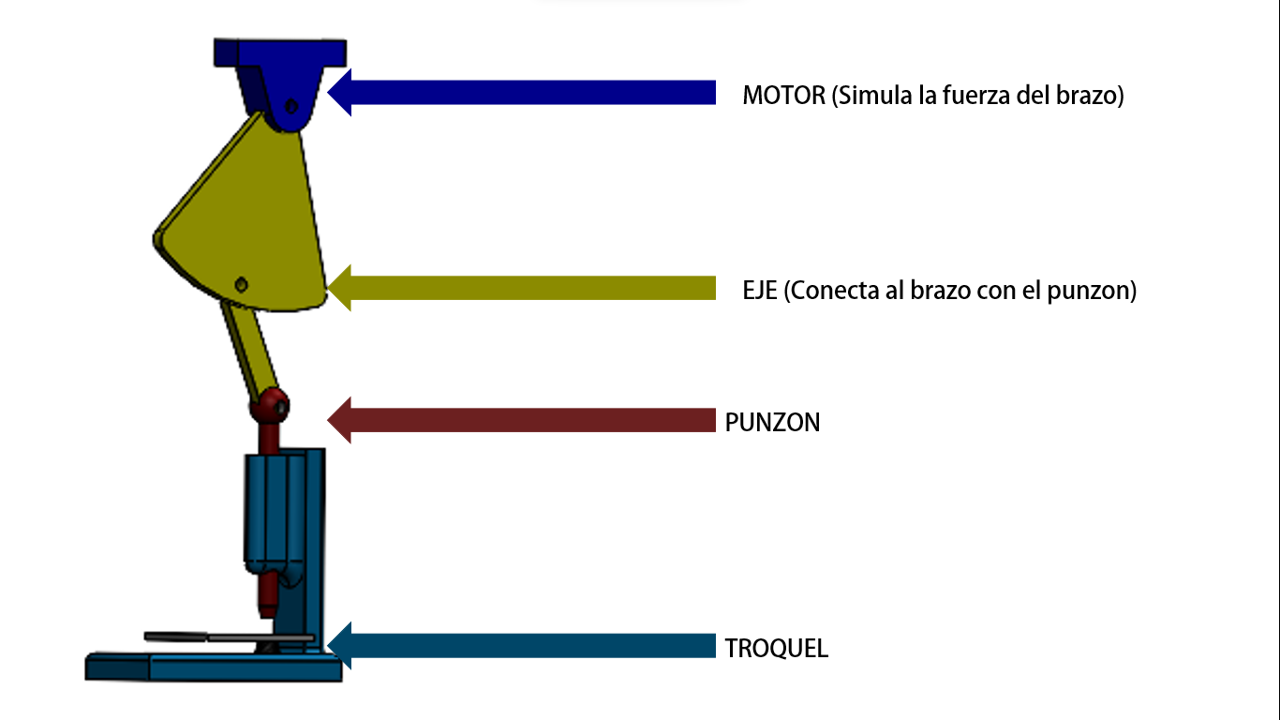
\includegraphics[width=0.8\textwidth]{Troquesolid.png}
    \caption{Troqueladora en SolidWorks}
    \label{fig:imagen3}
    \end{figure}
    \newpage
    \begin{itemize}
      \item Con SolidWorks Motion, es posible simular el movimiento de la máquina y su comportamiento dinámico bajo diferentes condiciones de carga. 
      \end{itemize}
      \begin{figure}[H]
      \centering
      
      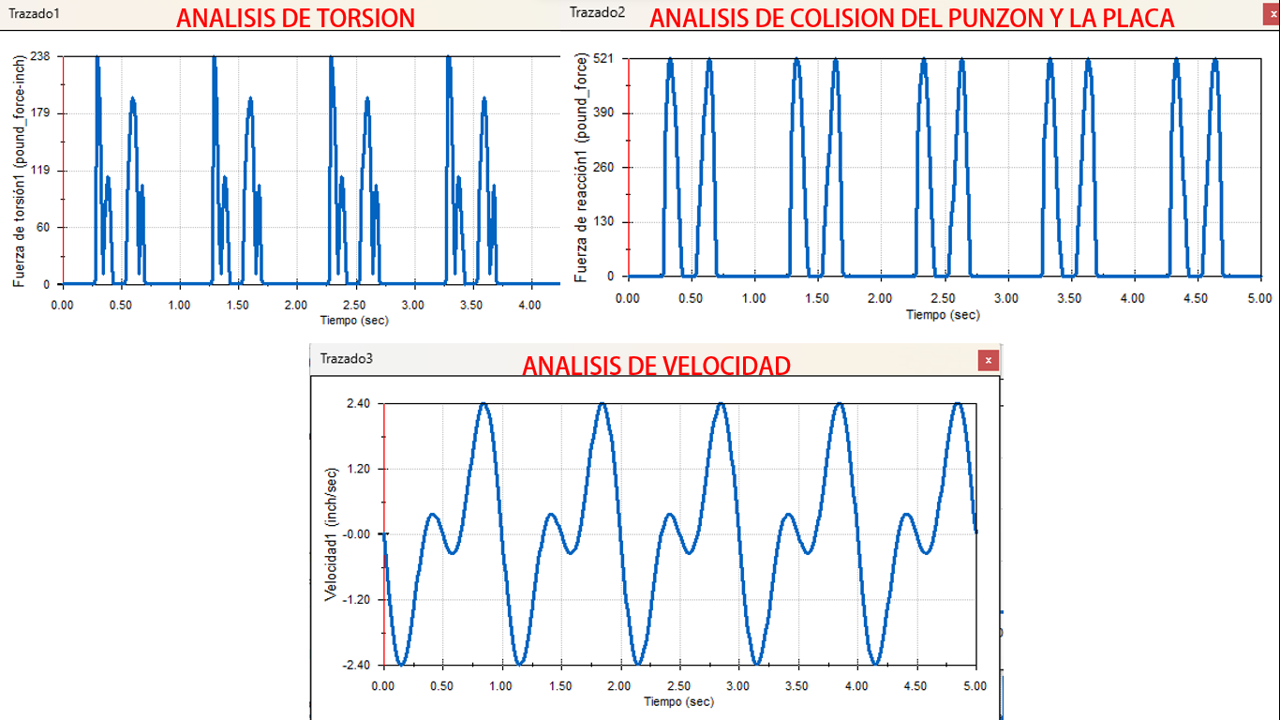
\includegraphics[width=0.8\textwidth]{Analisis1.png}
      \caption{Análisis dinámico}
      \label{fig:imagen3}
      \end{figure}
      \begin{itemize}
        \item Con SolidWorks Simulation, es posible realizar análisis de elementos finitos (FEA) para determinar las tensiones, deformaciones y factores de seguridad en la herramienta de corte y otras piezas importantes de la máquina.
        \end{itemize}
        \begin{figure}[H]
        \centering
        
        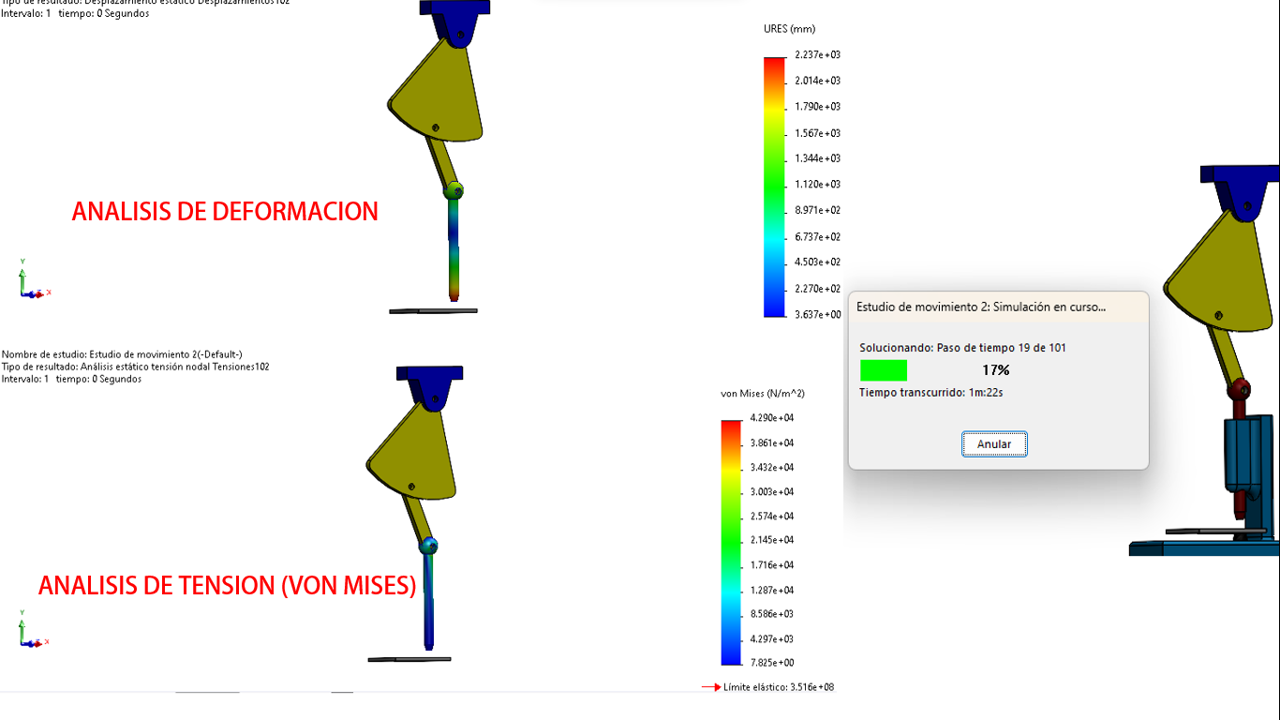
\includegraphics[width=0.8\textwidth]{Analisis2.png}
        \caption{Análsis de otras propiedades}
        \label{fig:imagen3}
        \end{figure}
    \newpage
    A continuación calcularemos:
    \begin{itemize}
        \item Fuerza de corte (Fc) 
     \newline
     Supongamos que queremos cortar una lámina de acero con un espesor de 3 mm y una longitud de corte de 20 cm, utilizando una herramienta de corte en forma de cuña. Si la constante K para el acero es de 0.8, podemos calcular la fuerza de corte necesaria de la siguiente manera:

        $$Fc = K * t * L$$
        $$Fc = 0.8 * 0.003 m * 0.2 m$$
        $$Fc = 0.00048 N$$
        \item Aceleración
        \newline
        Supongamos que la herramienta de corte que estamos utilizando en nuestra troqueladora manual tiene un diámetro de 8 cm y una velocidad de 5 m/s. Podemos calcular la aceleración de la herramienta de corte de la siguiente manera:
        $$ a = V^2 / r$$
        $$a = (5 m/s)^2 / 0.04 m$$
        $$a = 625 m/s^2$$
        \item Velocidad de la máquina (V)
        \newline
        Supongamos que la herramienta de corte que estamos utilizando en nuestra troqueladora manual tiene un diámetro de 5 cm y una velocidad de rotación de 1000 rpm. Podemos calcular la velocidad de la herramienta de corte de la siguiente manera:
        $$V = \pi * D * n / 60$$
        $$V = 3.1416 * 0.05 m * 1000 / 60$$
        $$V = 2.618 m/s$$
        \newpage
        \item Energía requerida (E)
        \newline
        Supongamos que queremos perforar un agujero en una lámina de acero con un espesor de 5 mm y un diámetro de 10 cm, utilizando una herramienta de corte en forma de broca. Si la fuerza de corte necesaria para perforar el acero es de 0.008 N, podemos calcular la energía requerida para el corte de la siguiente manera:

        $$E = Fc * d$$
        $$E = 0.008 N * \pi * (0.1 m)^2$$
        $$E = 0.0025 J$$
      \end{itemize}

        

    \section*{Conclusión}
    \addcontentsline{toc}{section}{Conclusiones}
    En conclusión, se logró estudiar el movimiento de una troqueladora y realizar cálculos empíricos de su velocidad, aceleración entre otras. Se construyó la máquina, sus troqueles y se realizaron experimentos para medir y demostrar conceptos de dinámica que afectan el funcionamiento de esta. 
    
    
    \newpage

    \section*{}
    \bibliographystyle{apacite}
    \nocite{*}
\bibliography{referencias}

\end{document}
